\documentclass[UTF8,12pt]{hue}

\begin{document}
	
	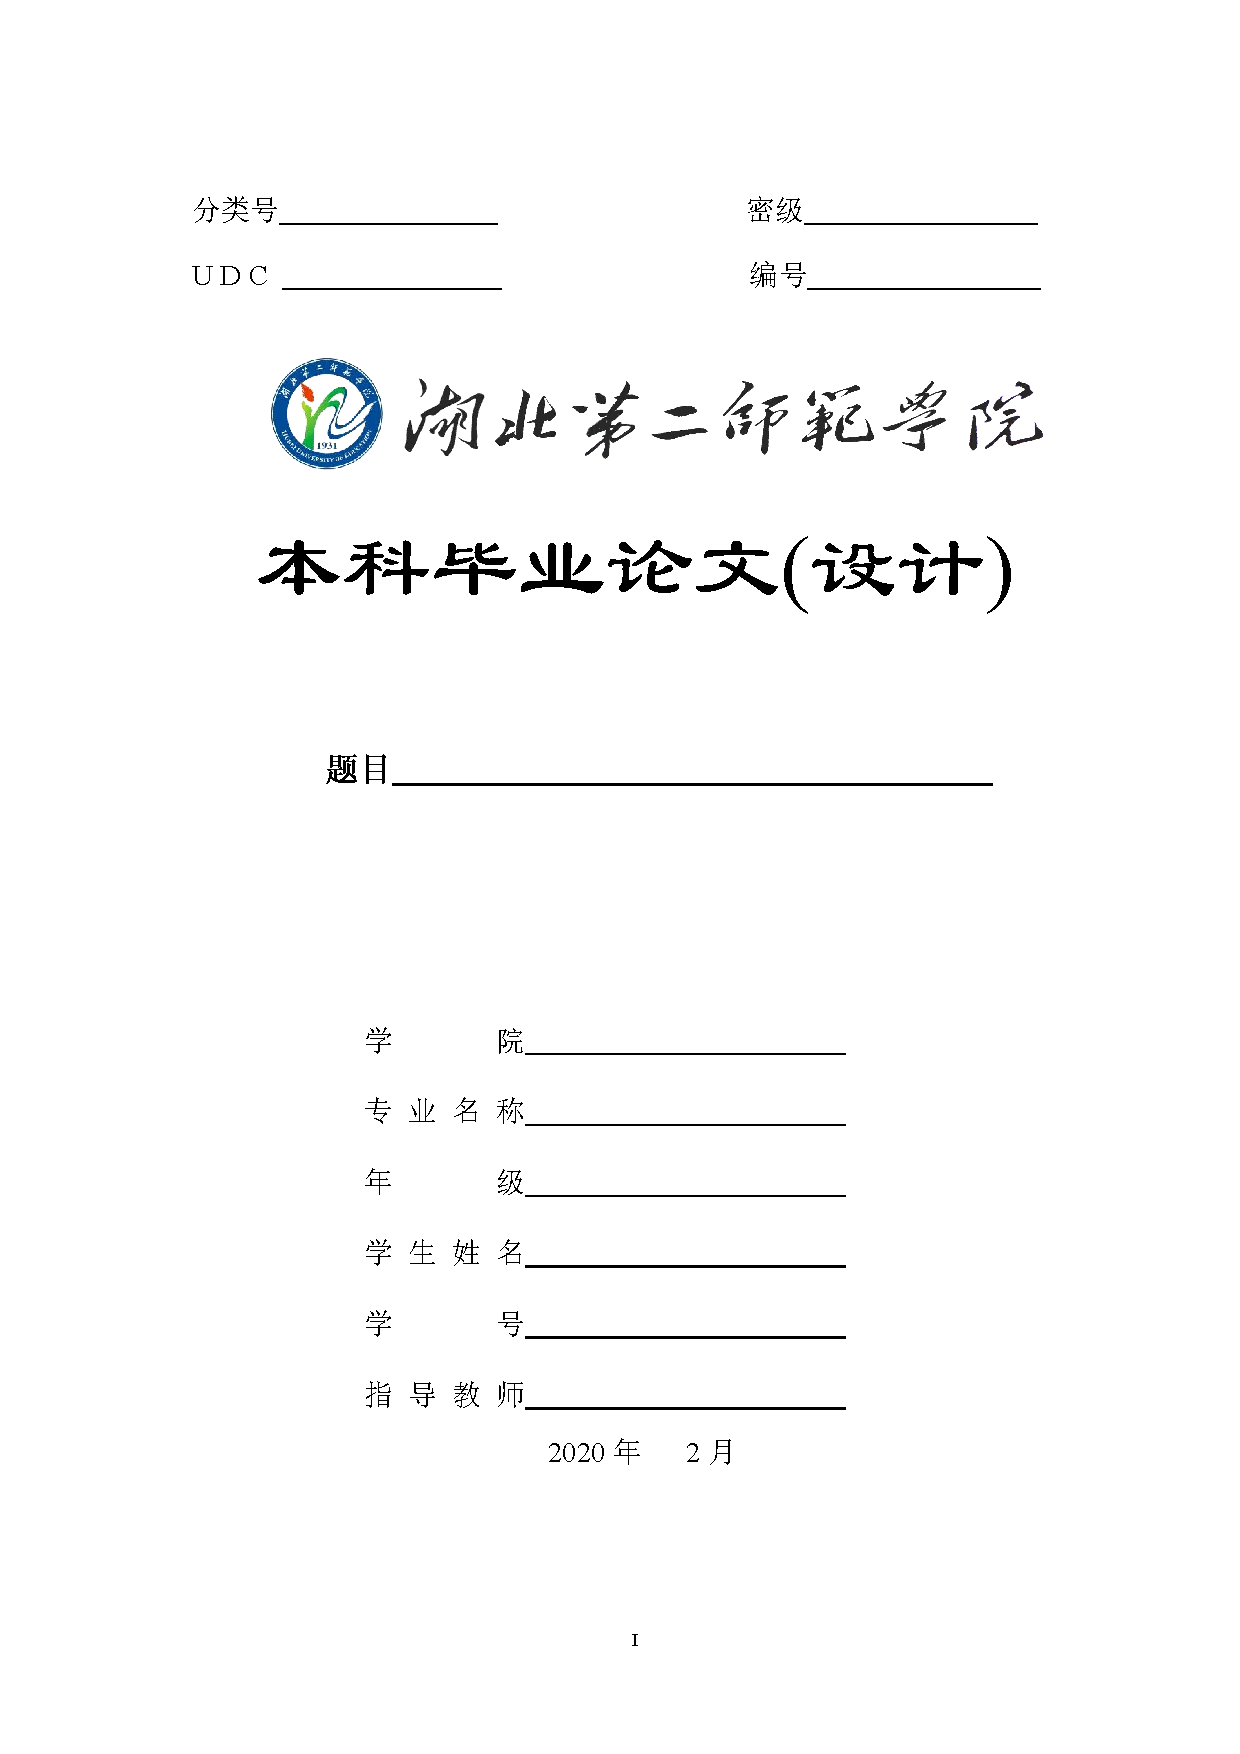
\includepdf{封面与承诺书/封面.pdf}
	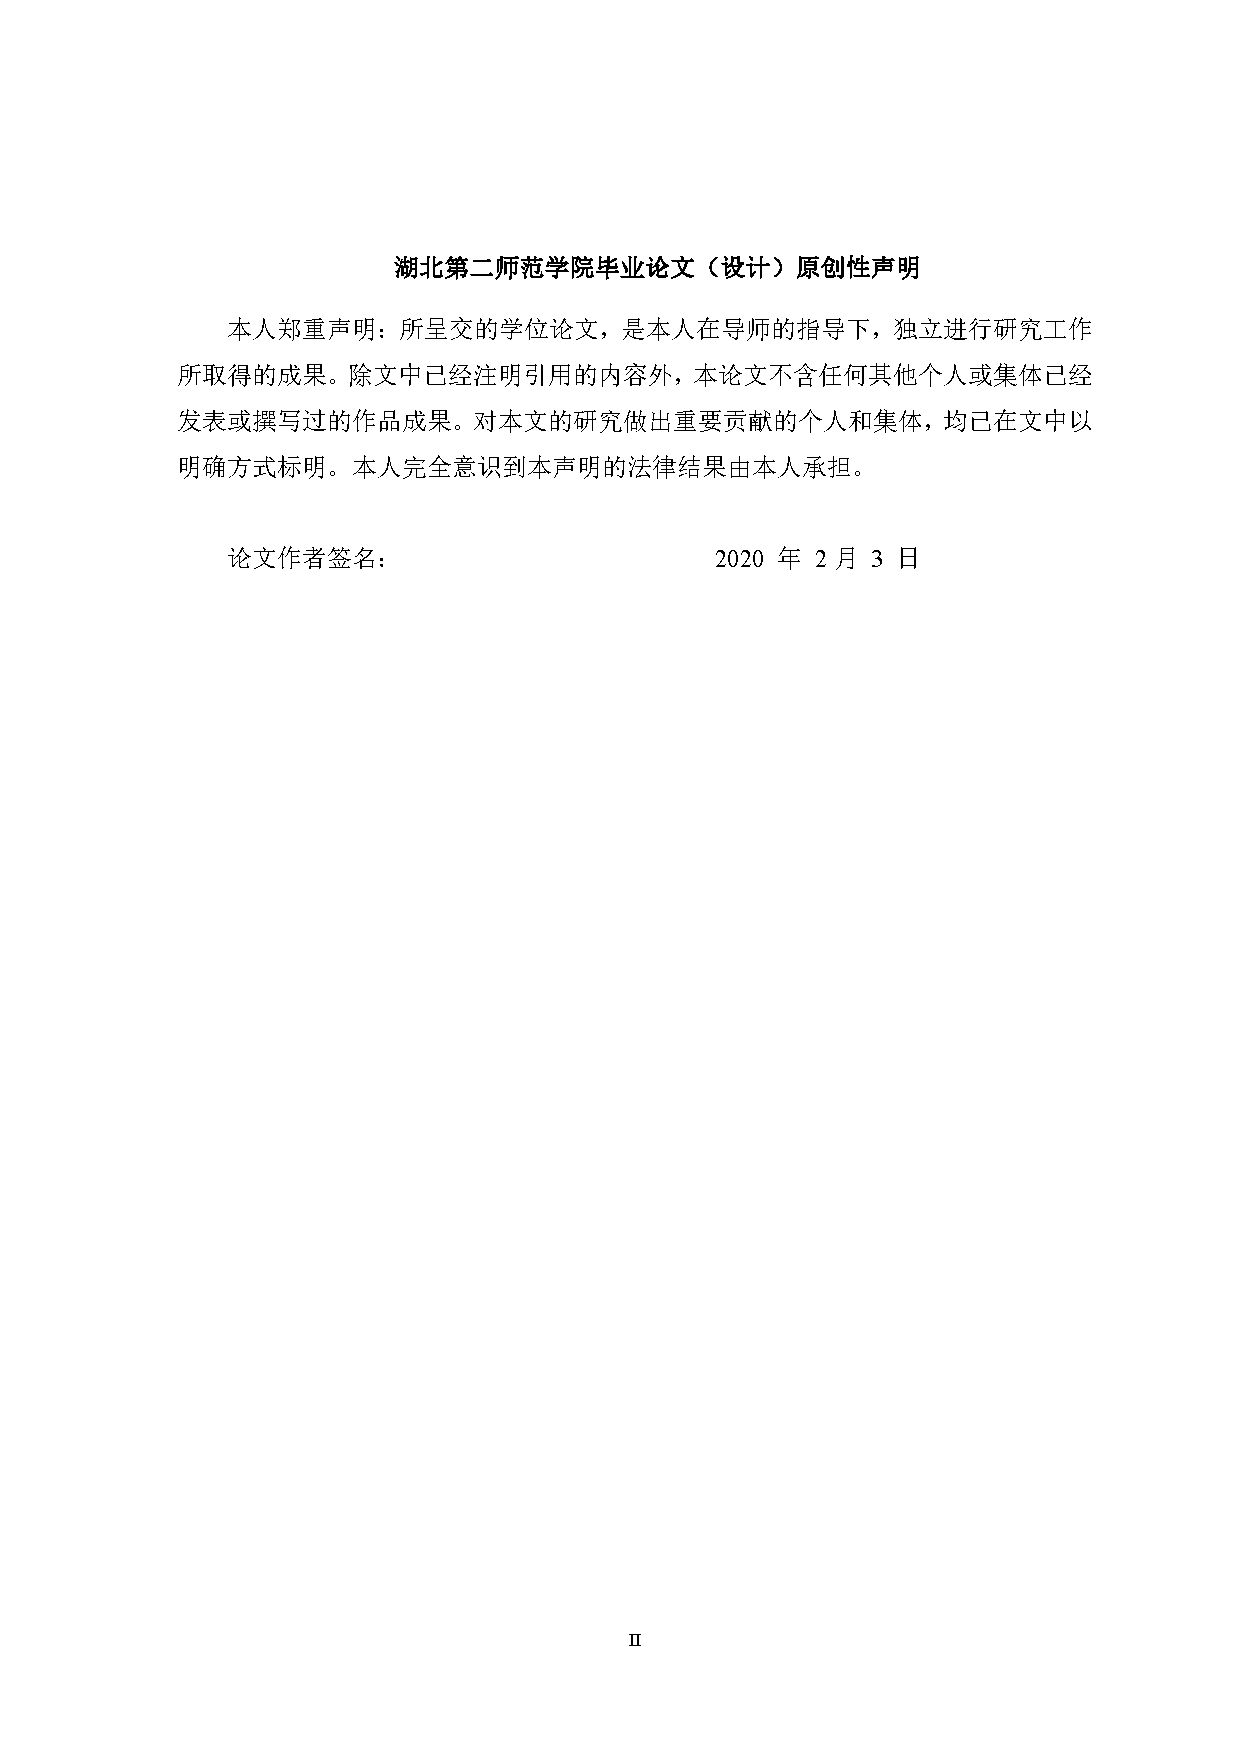
\includepdf{封面与承诺书/承诺书.pdf}
	
	\noindent\textbf{摘要:}中文摘要中文摘要中文摘要中文摘要中文摘要中文摘要中文摘要中文摘要中文摘要中文摘要中文摘要中文摘要中文摘要中文摘要中文摘要中文摘要中文摘要中文摘要中文摘要中文摘要中文摘要中文摘要中文摘要中文摘要中文摘要中文摘要中文摘要中文摘要中文摘要中文摘要中文摘要中文摘要中文摘要中文摘要中文摘要中文摘要中文摘要中文摘要中文摘要中文摘要中文摘要中文摘要中文摘要中文摘要中文摘要中文摘要中文摘要中文摘要中文摘要中文摘要中文摘要中文摘要中文摘要中文摘要中文摘要中文摘要中文摘要中文摘要中文摘要中文摘要中文摘要中文摘要中文摘要中文摘要中文摘要。

中文摘要中文摘要中文摘要中文摘要中文摘要中文摘要中文摘要中文摘要中文摘要中文摘要中文摘要中文摘要中文摘要中文摘要中文摘要中文摘要中文摘要中文摘要中文摘要中文摘要中文摘要中文摘要中文摘要中文摘要中文摘要中文摘要中文摘要中文摘要中文摘要中文摘要中文摘要中文摘要中文摘要中文摘要中文摘要中文摘要中文摘要中文摘要中文摘要中文摘要中文摘要中文摘要中文摘要中文摘要中文摘要中文摘要中文摘要中文摘要中文摘要中文摘要中文摘要中文摘要中文摘要中文摘要中文摘要中文摘要中文摘要中文摘要中文摘要中文摘要中文摘要中文摘要中文摘要中文摘要中文摘要。

中文摘要中文摘要中文摘要中文摘要中文摘要中文摘要中文摘要中文摘要中文摘要中文摘要中文摘要中文摘要中文摘要中文摘要中文摘要中文摘要中文摘要中文摘要中文摘要中文摘要中文摘要中文摘要中文摘要中文摘要中文摘要中文摘要中文摘要中文摘要中文摘要中文摘要中文摘要中文摘要中文摘要中文摘要中文摘要中文摘要中文摘要中文摘要中文摘要中文摘要中文摘要中文摘要中文摘要中文摘要中文摘要中文摘要中文摘要中文摘要中文摘要中文摘要中文摘要中文摘要中文摘要中文摘要中文摘要中文摘要中文摘要中文摘要中文摘要中文摘要中文摘要中文摘要中文摘要中文摘要中文摘要。



\vspace{1em}
\noindent\textbf{关键词:}关键词1~~ 关键词2~~ 关键词3~~ 关键词4~~ 关键词5~~ 关键词6\thispagestyle{empty}\newpage  
	\noindent\textbf{Abstract: }This is the English summary.This is the English summary. This is the English summary.This is the English summary.This is the English summary. This is the English summary.This is the English summary.This is the English summary. This is the English summary.This is the English summary.This is the English summary. This is the English summary.This is the English summary.This is the English summary. This is the English summary.This is the English summary.This is the English summary. This is the English summary.



This is the English summary.This is the English summary. This is the English summary.This is the English summary.This is the English summary. This is the English summary.This is the English summary.This is the English summary. This is the English summary.This is the English summary.This is the English summary. This is the English summary.This is the English summary.This is the English summary. This is the English summary.This is the English summary.This is the English summary. This is the English summary.


This is the English summary.This is the English summary. This is the English summary.This is the English summary.This is the English summary. This is the English summary.This is the English summary.This is the English summary. This is the English summary.This is the English summary.This is the English summary. This is the English summary.This is the English summary.This is the English summary. This is the English summary.This is the English summary.This is the English summary. This is the English summary.

\vspace{1em}
\noindent\textbf{Key Words: }Key Words; Key Words; Key Words; Key Words; Key Words; Key Words\thispagestyle{empty}\newpage  
	\begin{center}\tableofcontents|\end{center}\thispagestyle{empty}\newpage  
	
	\pagestyle{fancy}\setcounter{page}{1}
	\fancyhead{}\fancyfoot[R]{}\fancyfoot[L]{}
	

	\begin{center}\item\section{引言}\end{center}
	
	\subsection{问题背景}
	
	\subsection{问题提出}
	
	\subsection{问题分析}
	
	\begin{center}\item\section{文献综述}\end{center}
	
	\subsection{支持向量机}
	
	\subsection{决策树}
	
	\subsection{朴素贝叶斯}
	
	
	\begin{center}\item\section{符号说明}\end{center}
	
	\begin{center}\item\section{实验设计}\end{center}
	
	\begin{center}\item\section{实验过程}\end{center}
	
	\begin{center}\item\section{数据分析}\end{center}
	
	\begin{center}\item\section{结论}\end{center}
	
	\newpage\noindent\section*{参考文献}
	\addcontentsline{toc}{section}{参考文献} 
	
	
	\newpage\noindent\section*{致谢}
	\addcontentsline{toc}{section}{致谢}
\end{document} 